%%%%%%%%%%%%%%%%%%%%%%%%%%%%%%%%%%%%%%%%%%%%%%%%%%%%%
%				  Video In module					%
%					-----------						%
% Author: Vaibhav Singh	& Thibault Porteboeuf 		%
%%%%%%%%%%%%%%%%%%%%%%%%%%%%%%%%%%%%%%%%%%%%%%%%%%%%%

\section{VideoIn module}
\begin{figure}[H]
\center
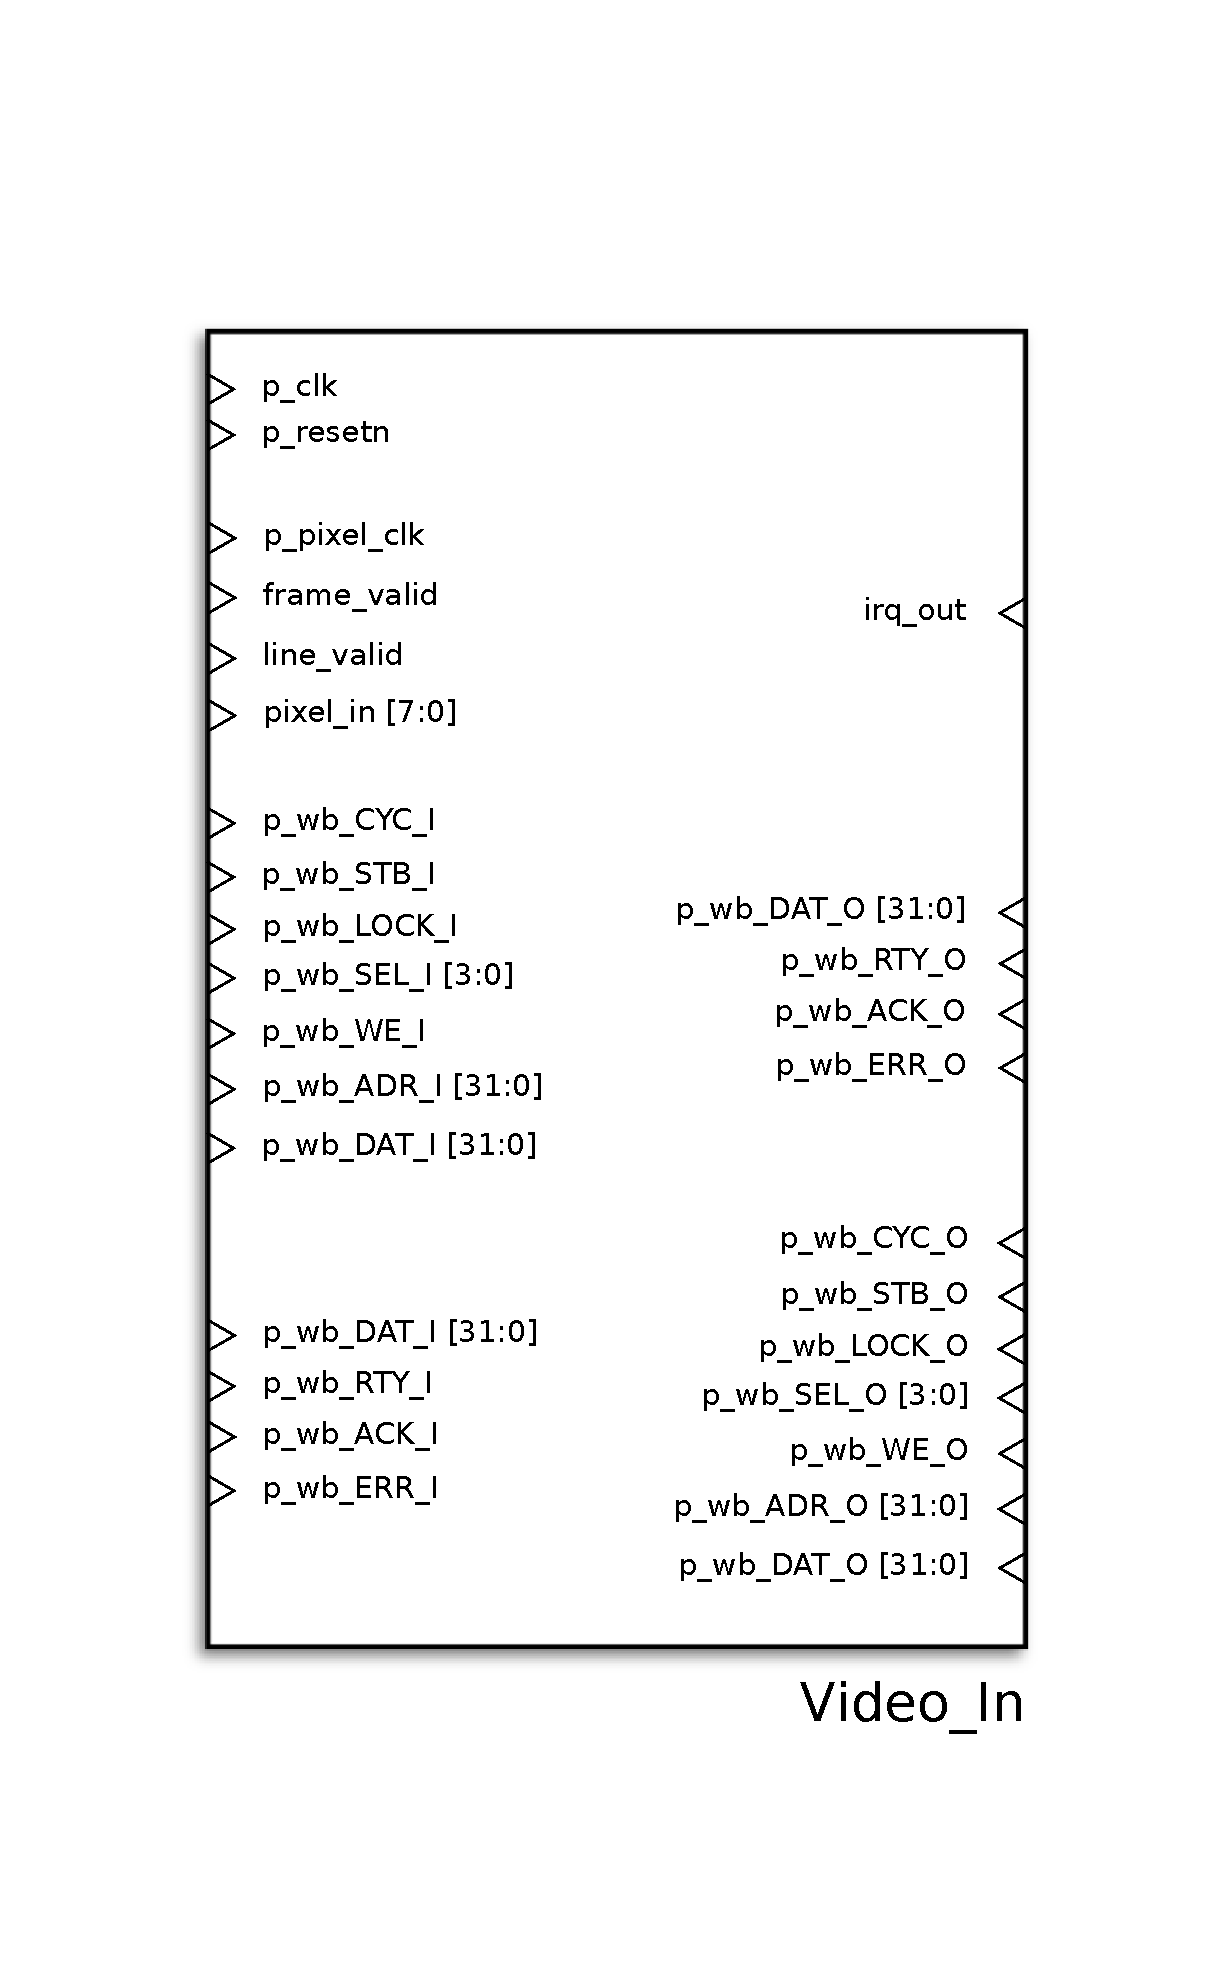
\includegraphics[width=7cm]{figs/Video_in.pdf}
\caption{VideoIn module's interface}
\label{VideoIn_interface}
\end{figure}

As explained before, VideoIn is the module responsible for handling the incoming video signals and transfer the frames to the memory over the whishbone bus.

As described in the figure below, Video In Module has two blocks, one that is responsible for handling the video signals and posting data using the master interface, and another one which is a one register slave, as described in section \ref{wb_reg_slave}.

The wishbone slave will handle incoming requests from the LM32, and store the content of write requests to its register. It is also responsible for driving the Irq wire, at the state machine's demand.
The slave will automatically acknowledge the Irq when a write request is received.

The state machine is in charge of the rest of the process.
It samples the configuration stored in the slave's register at every rising edge of the \texttt{frame\_valid} signal. Thus, the configuration is updated only at the beginning of a new frame.

It then posts data from the buffer to the RAM, starting at the previously given address. This process is illustrated in figure \ref{VideoIn_sm}.

\begin{figure}[h]
\center
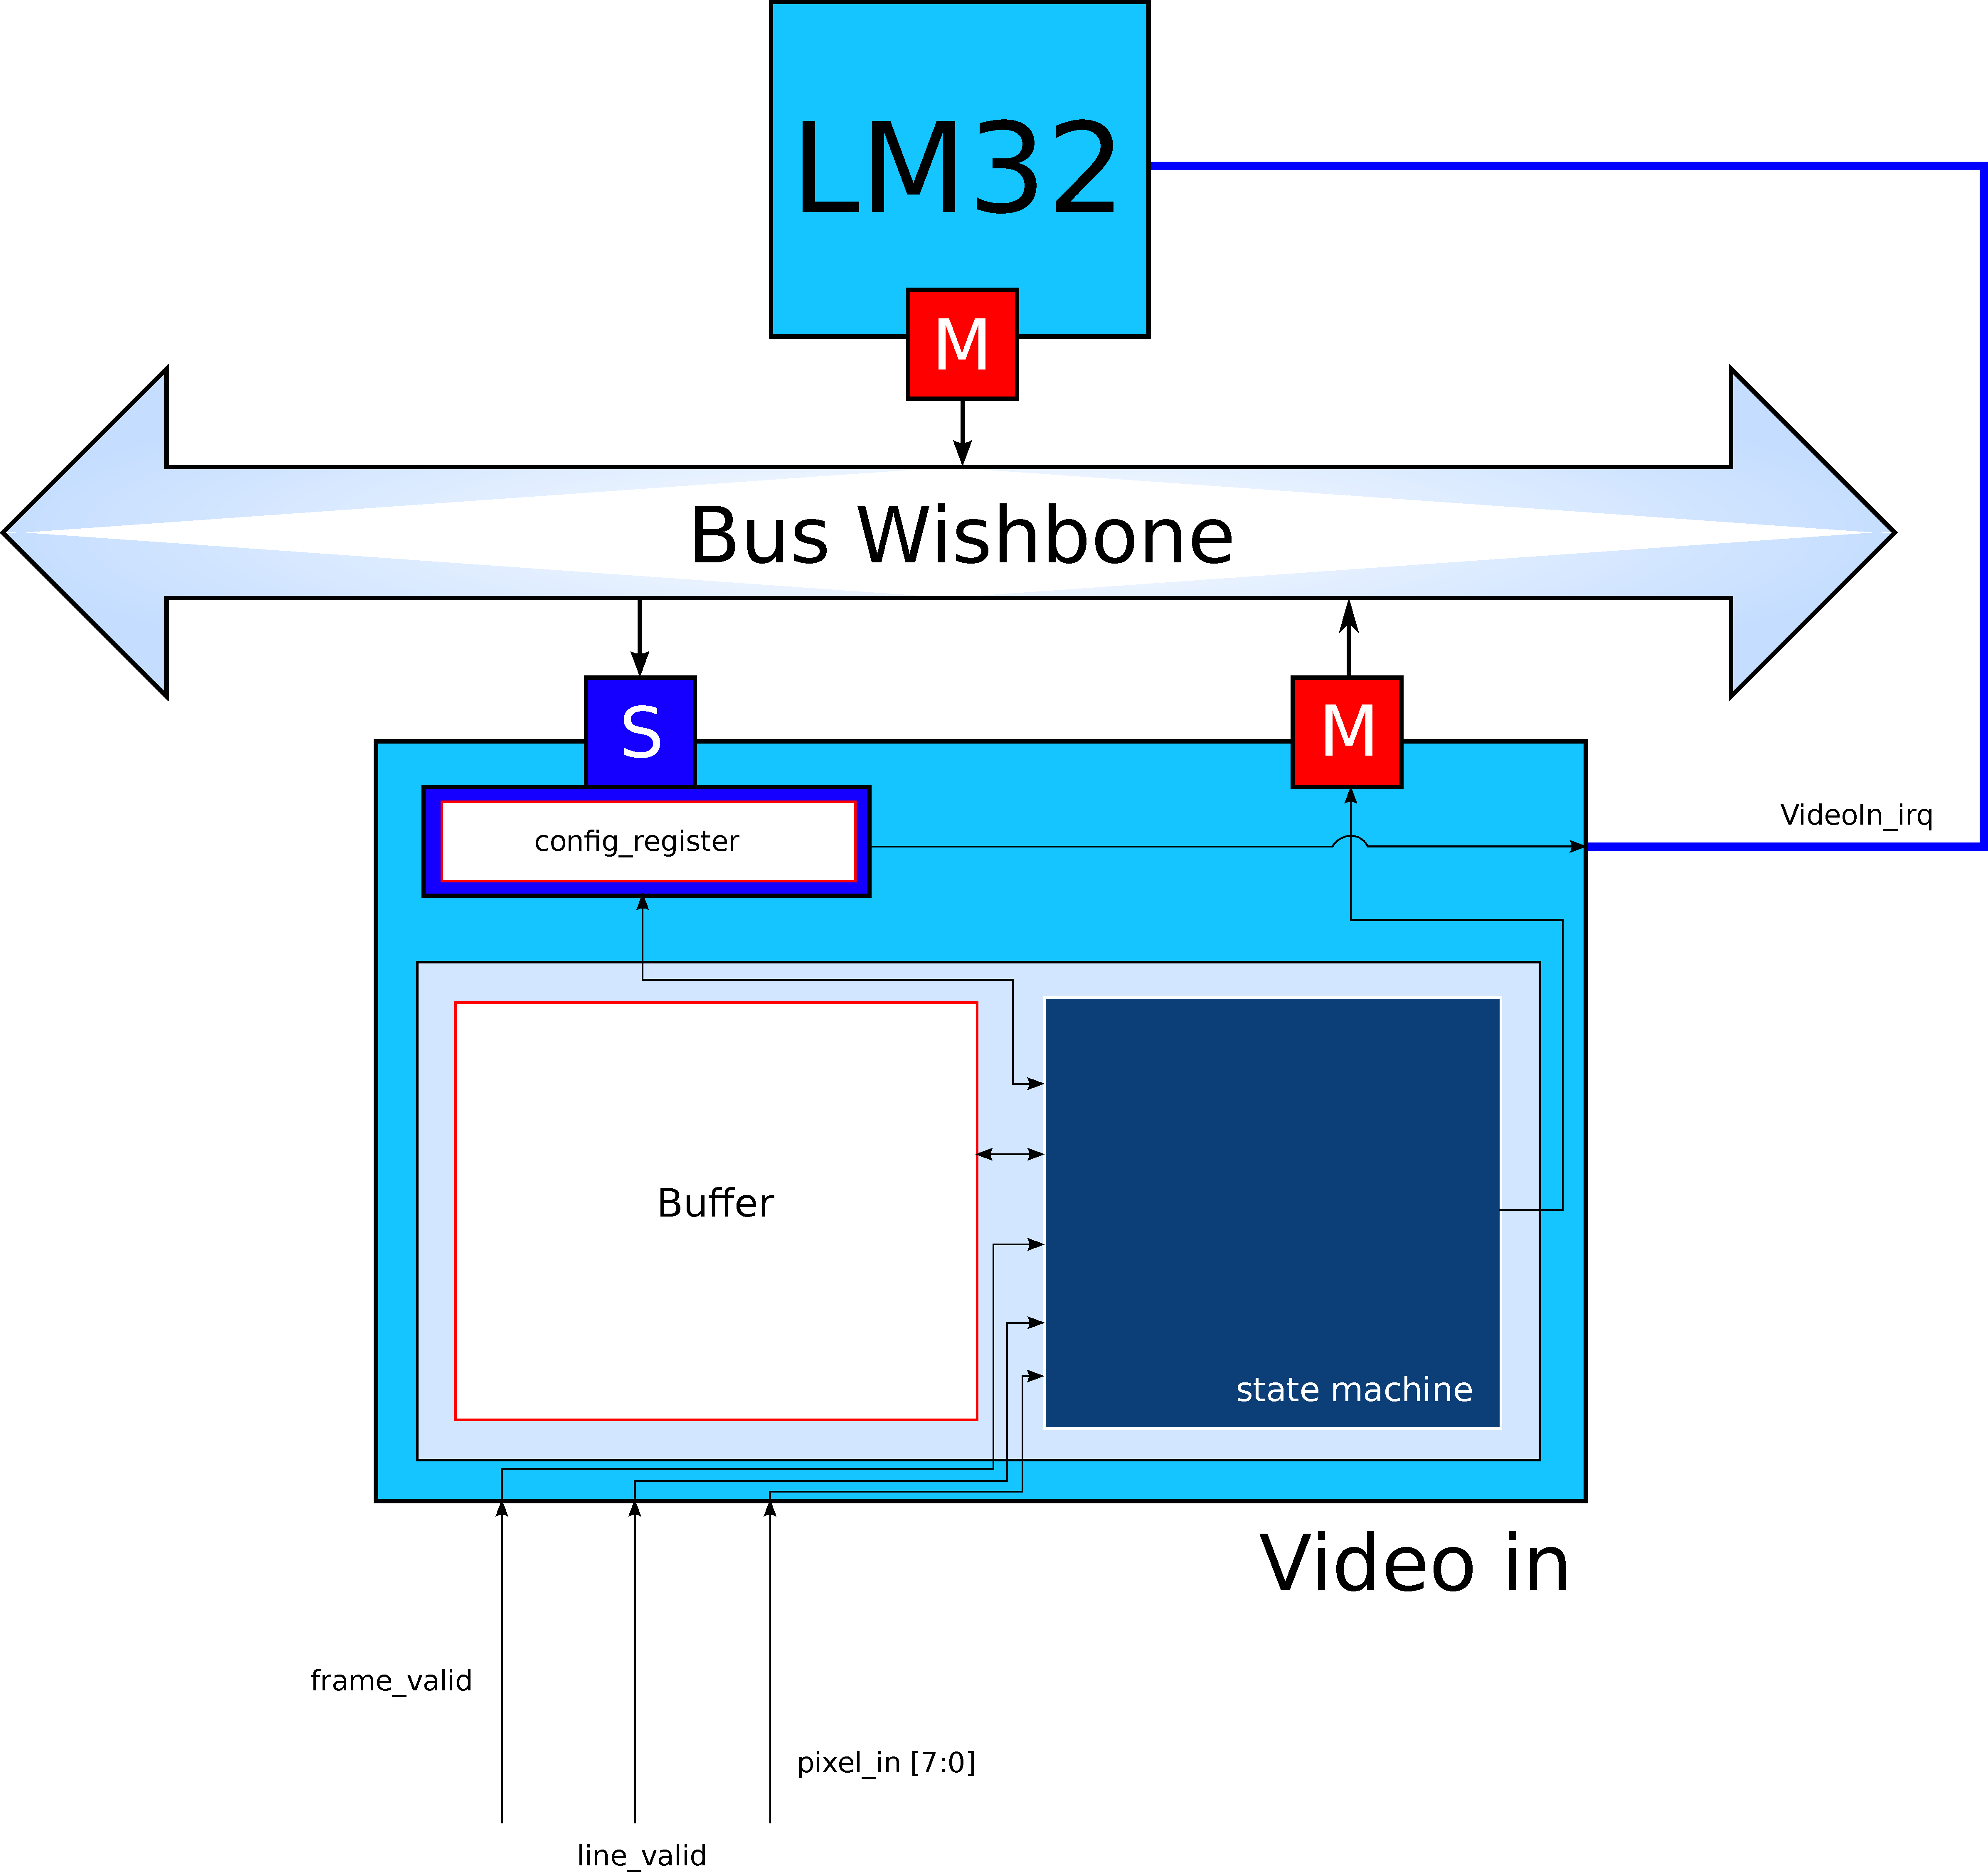
\includegraphics[width=11cm]{figs/Video_In_blocks.pdf}
\caption{VideoIn's inner structure}
\label{VideoIn_struct}
\end{figure}


\begin{figure}[h]
\center
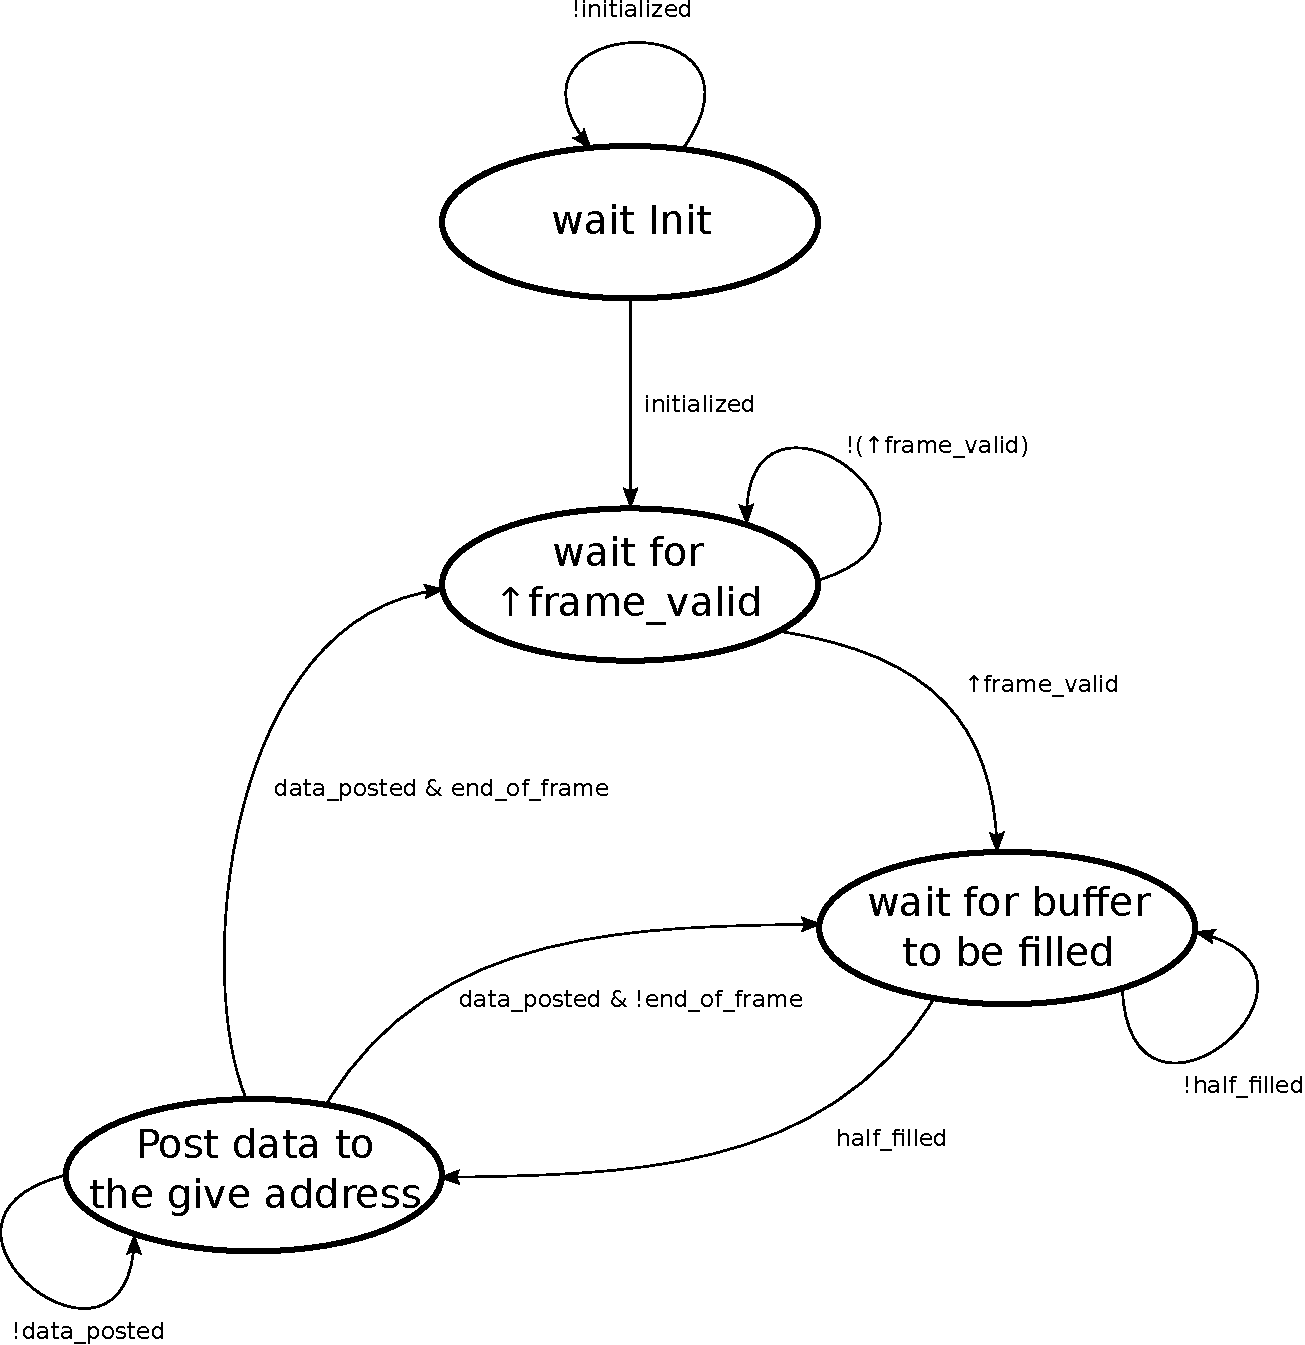
\includegraphics[width=11cm]{figs/video_in_sm.pdf}
\caption{VideoIn's behavior}
\label{VideoIn_sm}
\end{figure}

